% !TEX root = Projektdokumentation.tex
\section{Anhang}

\subsection{Beispielhafte Kommunikation über das gesamte System}\label{ExCom}
\begin{figure}[H]
\centering
\includegraphicsKeepAspectRatio{sequenceRegister.png}{1.0}
\caption{Beispielhafte Kommunikation über das gesamte System hinweg.}
\label{fig:KomGes}
\end{figure}

\subsection{Schaltplan}\label{Schaltplan}
%\subsubsection{Web Frontend: Übersicht der Räume}
\begin{figure}[H]
\centering
\includegraphicsKeepAspectRatio{schaltplan.png}{1.0}
\caption{Schaltplan}
\label{fig:schaltplan}
\end{figure}

\subsection{Platine}\label{Platine}
%\subsubsection{Web Frontend: Übersicht der Räume}
\begin{figure}[H]
\centering
\includegraphicsKeepAspectRatio{platine.png}{1.0}
\caption{Platine}
\label{fig:platine}
\end{figure}


\subsection{Screenshots vom Frontend}\label{FrontendScreens}
%\subsubsection{Web Frontend: Übersicht der Räume}
\begin{figure}[H]
\centering
\includegraphicsKeepAspectRatio{Rooms.png}{1.0}
\caption{Web Frontend: Übersicht der Räume}
\label{fig:FE_Rooms}
\end{figure}

\subsubsection{Web Frontend: Ein neuer Raum wurde registriert}
\begin{figure}[H]
\centering
\includegraphicsKeepAspectRatio{NewRoom.png}{1.0}
\caption{Web Frontend: Ein neuer Raum wurde registriert}
\label{fig:FE_NewRoom}
\end{figure}

\subsubsection{Web Frontend: Übersicht der Geräte eines Raums}
\begin{figure}[H]
\centering
\includegraphicsKeepAspectRatio{Devices.png}{1.0}
\caption{Web Frontend: Übersicht der Geräte eines Raums}
\label{fig:FE_Devices}
\end{figure}

\subsubsection{Web Frontend: Lichtschalter}
\begin{figure}[H]
\centering
\includegraphicsKeepAspectRatio{Switch.png}{1.0}
\caption{Web Frontend: Lichtschalter}
\label{fig:FE_Switch}
\end{figure}

\subsubsection{Web Frontend: Heizung}
\begin{figure}[H]
\centering
\includegraphicsKeepAspectRatio{Heating.png}{1.0}
\caption{Web Frontend: Heizung}
\label{fig:FE_Heating}
\end{figure}

\subsubsection{Web Frontend: Ändern der Temperatur}
\begin{figure}[H]
\centering
\includegraphicsKeepAspectRatio{ValueChange2.png}{1.0}
\caption{Web Frontend: Ändern der Temperatur}
\label{fig:FE_Change}
\end{figure}


\subsubsection{Konfigurationsseite des Raumservers}
\begin{figure}[H]
\centering
\includegraphicsKeepAspectRatio{Config.png}{1.0}
\caption{Konfigurationsseite des Raumservers}
\label{fig:ConfigRaum}
\end{figure}



\begin{figure}[H]
\centering
\includegraphicsKeepAspectRatio{ConfigLogin.png}{1.0}
\caption{Eingabemaske für den Cloud Account}
\label{fig:ConfigRaum_Login}
\end{figure}


\subsubsection{Aufspielen der Software auf den Atmega88}
\begin{figure}[H]
\centering
\includegraphicsKeepAspectRatio{flashing.jpg}{1.0}
\caption{Aufspielen der Software auf den Atmega88}
\label{fig:Flashing}
\end{figure}




%\subsection{Detaillierte Zeitplanung}
%\label{app:Zeitplanung}
%\tabelleAnhang{ZeitplanungKomplett}

%\subsection{Gantt-Diagramm}
%\label{app:Gantt}
%\begin{sideways}
%\begin{ganttchart}[
hgrid,
vgrid,
x unit=4mm,
time slot format=isodate
]{2016-04-12}{2016-05-31}
\gantttitlecalendar{year, month, day, week=3, weekday} \\

\ganttbar{}{2016-04-14}{2016-04-17}

\end{ganttchart}

%\end{sideways}
\subsection{API Dokumentation}\label{API_Doc}

\subsubsection{API Aufruf: Registrieren eines neuen Benutzers}
\label{app:API_register}
\tabelleAnhang{WebService/register}

\subsubsection{API Aufruf: Als registrierter Benutzer anmelden}
\label{app:API_login}
\tabelleAnhang{WebService/login}

\subsubsection{API Aufruf: Einen Raum registrieren}
\label{app:API_register_room}
\tabelleAnhang{WebService/newRoom}

\subsubsection{API Aufruf: Einen Raum von der Datenbank entfernen}
\label{app:API_delete_room}
\tabelleAnhang{WebService/deleteRoom}

\subsubsection{API Aufruf: Einen spezifischen Raum abrufen}
\label{app:API_show_room}
\tabelleAnhang{WebService/getRoom}

\subsubsection{API Aufruf: Eine Liste aller Räume abrufen}
\label{app:API_show_rooms}
\tabelleAnhang{WebService/getRooms}

\subsubsection{API Aufruf: Ein neues Gerät registrieren}
\label{app:API_register_device}
\tabelleAnhang{WebService/registerDevice}

\subsubsection{API Aufruf: Ein spezifisches Gerät abrufen}
\label{app:API_get_device}
\tabelleAnhang{WebService/getDevice}

\subsubsection{API Aufruf: Ein Gerät aus der Datenbank entfernen}
\label{app:API_delete_device}
\tabelleAnhang{WebService/deleteDevice}

\subsubsection{API Aufruf: Alle Geräte eines Raumes auflisten}
\label{app:API_show_devices}
\tabelleAnhang{WebService/getDevices}

\subsubsection{API Aufruf: Verändern der Gerätedaten}
\label{app:API_patch_device}
\tabelleAnhang{WebService/patchDevice}




%\subsection{Projektdokumentation Sommersemester 2015}
%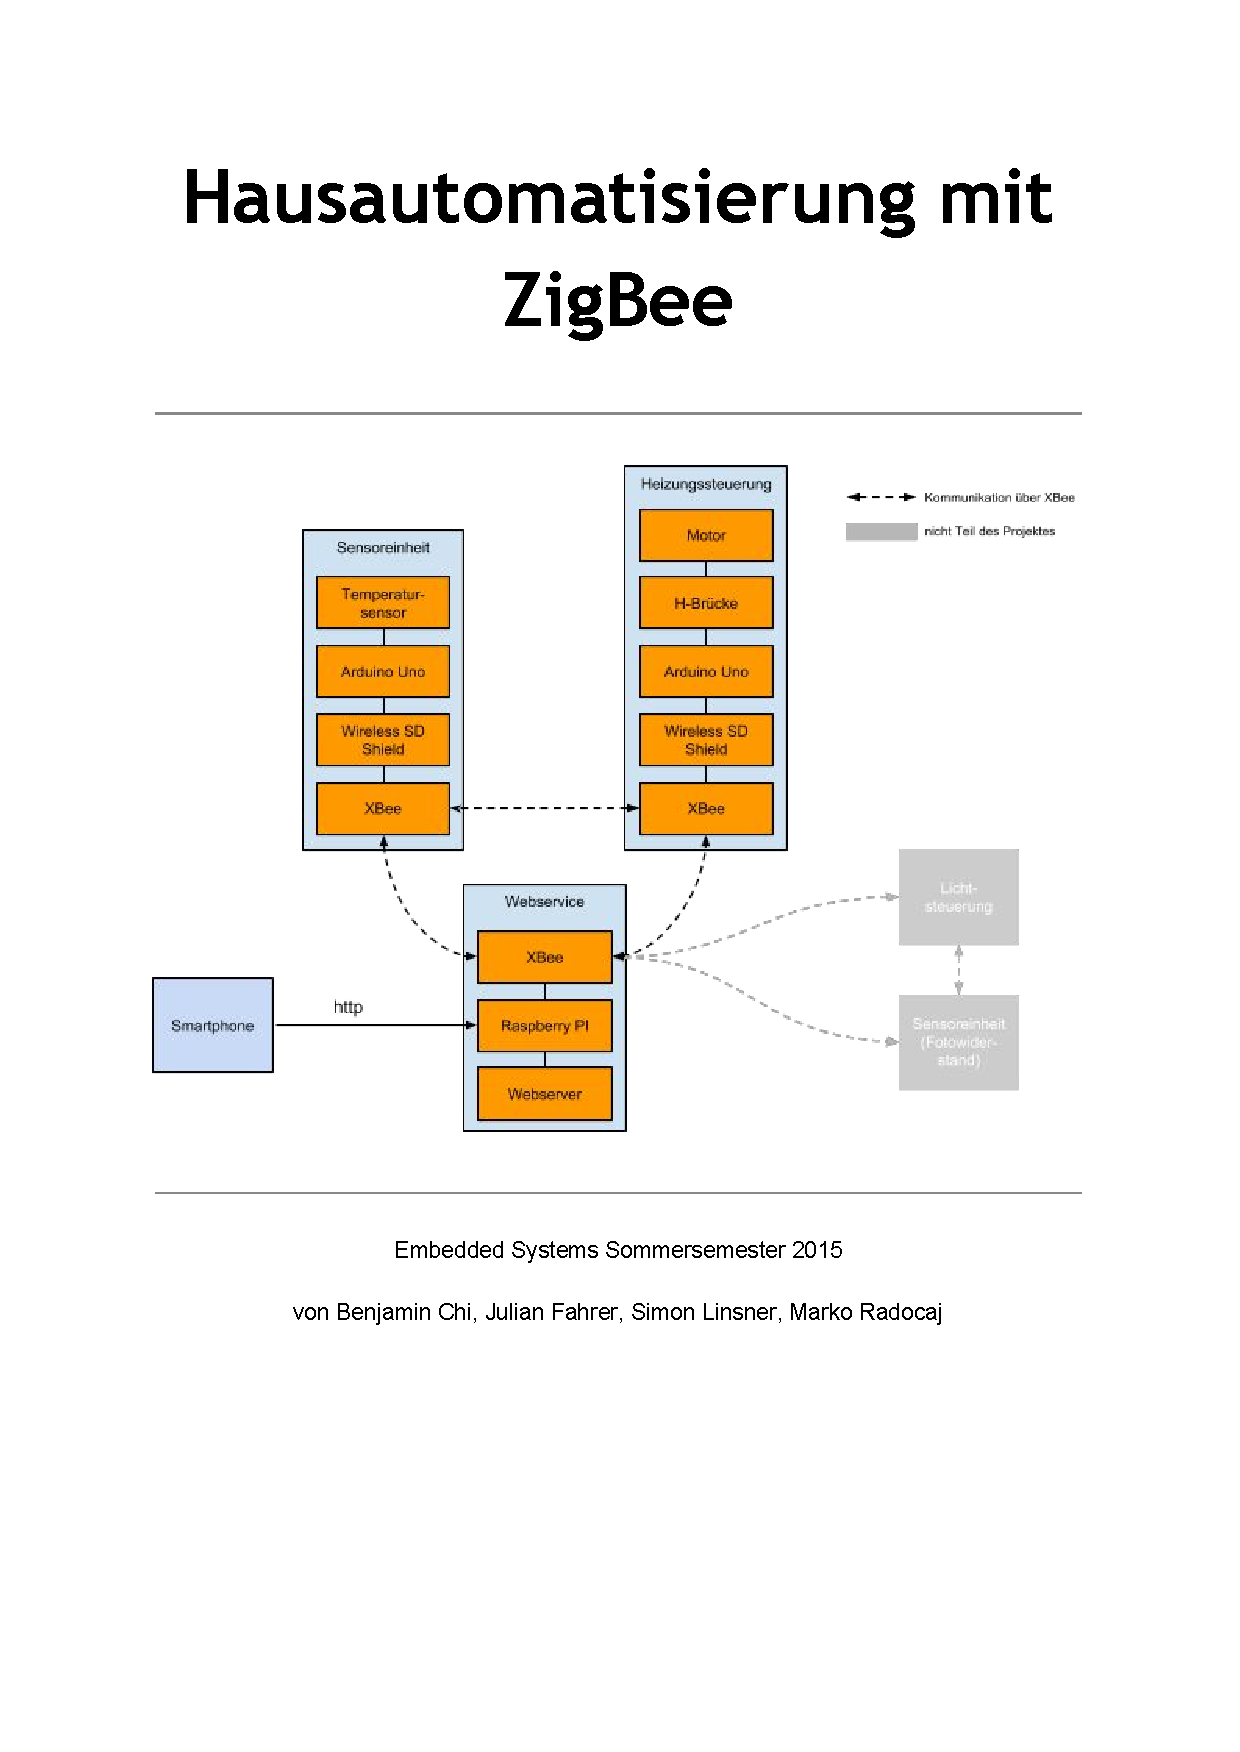
\includepdf[pagecommand={\thispagestyle{headings}},
%  pages=1-23, scale=0.8, frame=true]{Anhang/Dokumentation_SoSe2015.pdf}

